\chapter{Approach}
\label{chap:approach}
This chapter introduces the distinctive concept of a configurable search engine and outlines the comprehensive software architecture. It thoroughly explores and showcases all the required components for constructing the search engine, along with discussing implementation specifics. This encompasses the pivotal models and classes employed for the components and algorithms.
Furthermore, the chapter delves into the user interface, clarifying how it enhances user experience and facilitates configuring the search engine.

\section{Software Architecture}

Figure 4 provides an overview of the software architecture employed by the search engine. Microservices architecture was used to make scalability easier and also to split the responsibilities of each component. Docker is used to enforce this architectural pattern where the Ubuntu:18.04 image is used for each component. Below is a compilation of the utilized technology stack:

\begin{figure}[h]	
     \centering
     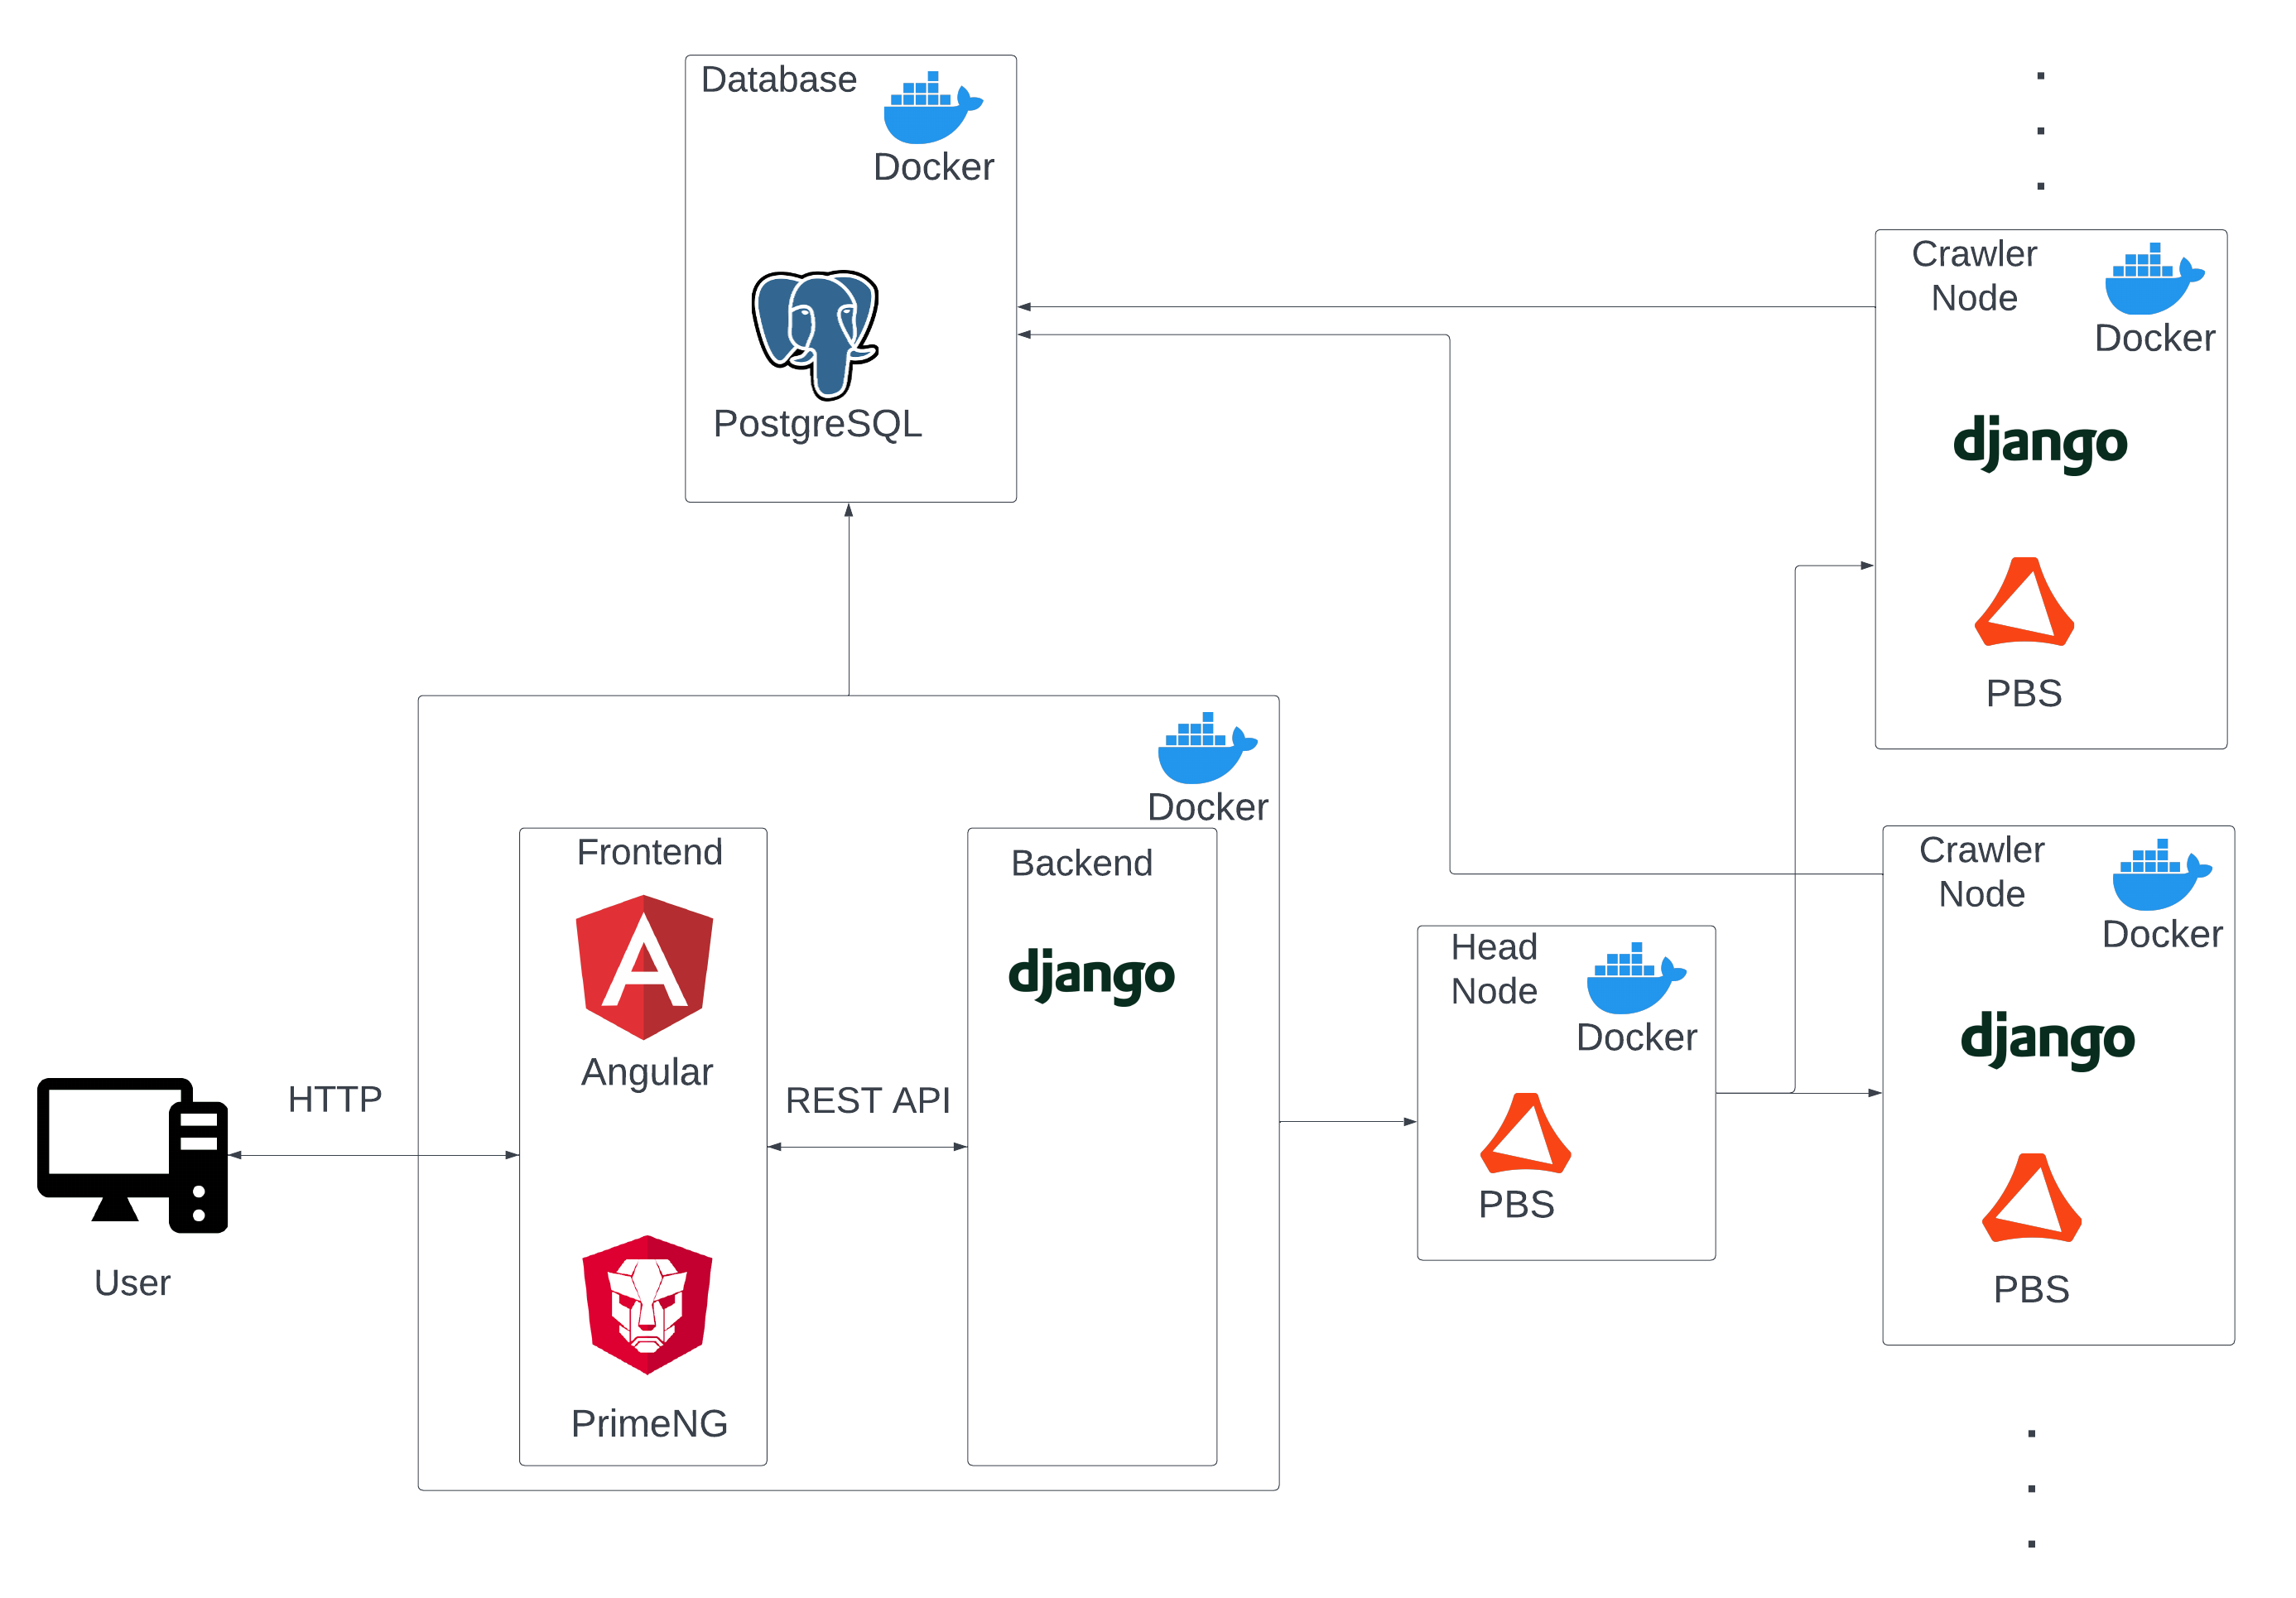
\includegraphics[width=10cm]{images/software_arch.png}
     \caption{High-level view of the software archtiticture.}
     \label{fig:software-arch}
\end{figure}

\begin{itemize}
  \item \textbf{Frontend (Angular \& PrimeNG)}: Positioned closest to the user, this component encompasses all pages and views. Angular is leveraged in conjunction with the contemporary CSS library, PrimeNG. To communicate with the backend, it employs the REST API.
  \item \textbf{Backend (Django)}: Serving as the core intelligence of the search engine, the backend houses both the crawler and indexer modules. It facilitates interaction with the Head node to initiate crawling based on user-defined configurations. Moreover, it establishes a connection with PostgreSQL for the storage of crawler and indexer configurations, along with job-related information.
  \item \textbf{Head Node (PBS)}: Operating as the central hub, this node orchestrates job management and determines the allocation of tasks to Crawler nodes, which are responsible for traversing the specified websites.
  \item \textbf{Crawler Node (PBS)}: These instances are designated to execute the crawling process and store the resulting data in the PostgreSQL database.
\end{itemize}

The application setup initiates with a minimal requirement of four microservices to operate the entire search engine. One Docker container containing both Angular and Backend logic must establish connections with two other containers: the Database and PBS Head Node. The PBS Head Node, in turn, should connect to one or more Crawler Node containers responsible for executing the crawling task. The Crawler Node will perform the crawling job and save the results to the shared Database.

The workflow begins with a user-friendly interface presented by Angular and PrimeNG, encompassing all the configurations and tools enabling users to crawl quickly and index various websites. Users can modify configurations and submit a crawling job to the Head Node. The Head Node, in response, identifies an available Crawler Node to execute the task. It's worth noting that the PBS cluster can be bypassed, and the crawling process can be run locally on a localhost server. Users can monitor the progress of the running job from the browser. Once crawling is completed and the user is happy with the result, the user can start indexing. The indexing job also does not support a distributed architecture and will be executed locally and not on the PBS cluster.


\subsection{Crawler Implmentation}

PBS Crawler Node runs the crawling job or can also run locally. The job supports multithreading. As illustrated by the pseudo-code shown in Algorithm [1], the crawler starts by loading the configuration submitted by the user from the Database. More details about the configuration are in the user interface section. Based on the configuration of a thread pool, the number of threads is read by the configuration. The thread pool contains all the threads crawling the site, where each thread contains a queue of URLs that it crawls from. The thread pool makes sure that if one thread has no URLs anymore, it can ask other threads to help. Algorithm [2] explains how this sharing URLs mechanism works. 

A seed URL is added to the current thread queue. The seed URL represents the starting point for the crawling, and the user configuration defines it. Using the sead url, the robots.txt content is downloaded once and can be reused for the rest of the crawling process.    

Each thread goes into an infinite loop that will continue to run either if the URLs queue still contains URLs to be fetched or at least one thread is still running. This guarantees that although one thread is running, it can be that that thread contains a lot of URLs that need help with crawling, and the free threads can share the load with it. If the thread queue is empty, it will ask the pool to find the next URLs to fetch. Otherwise, the first URL in the queue will be fetched, and a request using Selenium will be made. Afterwards, automated actions such as scrolling down, waiting and clicking defined by the user are executed. Those actions give the power to control the browser by the user to mimic real agent behaviour. The action chain will be discussed more in the User Interface section.  

After the page is rendered and the automated actions are executed, the next step is to collect the next URLs and add them to the URLs queue. The last step is to parse the documents needed from the page and filter the duplicated documents. 


\begin{algorithm}[h]
	\caption{$Start Crawling$}\label{alg:alg1}
	\begin{algorithmic}[1]
		\State $load\_crawler\_configurations()$
		\State $thread$ $\gets$ $create\_threads\_pool()$
	    \State $urls\_queue$ $\gets$ $get\_thread\_urls\_queue(thread)$
	    \State $seed\_url$ $\gets$ $get\_seed\_url()$
	    \State $sdd\_ulr\_to\_queue(urls\_queue, seed\_url)$
	    \State $robot\_file$ $\gets$ $get\_robot\_file\_content()$
	    \While {$urls\_queue$ not empty or All threads not done}
		\If{$urls\_queue$ is empty}
		    \State $urls\_queue$ $\gets$ $get\_thread\_urls\_queue(thread)$
		\Else
			\State $current\_url$ $\gets$ $urls\_queue.pop()$
			\State $filter\_unwanted\_urls(current\_url)$
			\State $request\_page(current\_url)$
            \State $execute\_automated\_actions()$
			\State $find\_next\_urls\_and\_add\_them\_to\_urls\_queue()$
			\State $docs$ $\gets$ $find\_and\_download\_targeted\_documents()$
			\State $filter\_unwanted\_documents(docs)$
		\EndIf
		\EndWhile

	\end{algorithmic}
\end{algorithm}

\subsection{Indexer Implmentation}